% =====================================================================
%  Paper 2 — RetinAI v3 + v4. IEEE two-column (IEEEtran, conference layout).
%  Build:  tectonic -X compile paper2_pretraining.tex   (figures in ./figs2/, drawn by scripts/paper2_figures.py)
%  Word:   .venv/bin/python scripts/make_paper_docx.py --paper2   (-> RetinAI_Paper2_Pretraining_draft.docx)
%  Every number traces to results/rop/v3/{v3_scores.json, report_data.json} (data commit b827cce),
%  results/prepared/rop_staging/v4/v4_summary.json, results/rop/v4/audit/audit_summary.json and
%  docs/v4/V4_MODEL_REPORT.md (fold-level AP-ROP recall). Items in \FILL{...} must be completed by the authors.
% =====================================================================
\documentclass[conference]{IEEEtran}
\usepackage{graphicx,booktabs,amsmath,amssymb,xcolor,url}
% IEEEtran asks for Times (ptm); under XeTeX/Tectonic the Type 1 ptm shapes are missing and bold/italic silently
% fall back to Latin Modern Regular, so load the OpenType Times clone explicitly.
\usepackage{fontspec}
\setmainfont{texgyretermes}[Extension=.otf,UprightFont=*-regular,BoldFont=*-bold,ItalicFont=*-italic,BoldItalicFont=*-bolditalic]
\graphicspath{{figs2/}}
\newcommand{\FILL}[1]{\textcolor{red}{\textbf{[FILL: #1]}}}
\IEEEoverridecommandlockouts

\title{Pre-training Domain, Data Cleaning and Training Recipe for Eye-Level ICROP-3 Staging of Retinopathy of Prematurity: A Pre-Registered Nine-Arm Comparison across Four Hospitals}

\author{\IEEEauthorblockN{Praharsh Nagpure, \FILL{R. Bait full name}, \FILL{P. Rangnekar full name},\\ \FILL{Y. Shengale full name}, and \FILL{A. Kumar full name}}
\IEEEauthorblockA{Department of Automation and Robotics, Vivekanand Education Society's Institute of Technology, Mumbai, India\\
Corresponding author: \FILL{name, e-mail, ORCID}}}

\begin{document}
\maketitle

\begin{abstract}
Retinopathy of prematurity (ROP) is a leading preventable cause of childhood blindness, and automated staging could extend scarce expert readers. Many published systems report 95--99\% accuracy within one cohort, some from splits made by photograph; performance at an unseen hospital is rarely measured. Under a protocol pre-registered before training, we compared nine arms for six-class ICROP-3 staging: retinal (RETFound-Green) versus natural-image (DINOv2) pre-training of one ViT-S/14 under one recipe, an EfficientNetV2-S baseline, an ensemble, native resolution, unsupervised adaptation, examination-level training and, in a final round, a quality-audited training pool alone and with a regularising recipe. Arms trained on 6{,}700 photographs of 1{,}528 infants from three hospitals with patient-grouped cross-validation and were scored per eye at a fourth hospital (230 eyes). The selection rule chose DINOv2 (cross-validation quadratic weighted kappa 0.825, 95\% CI 0.737--0.911); neither the audited pool nor the recipe reached the pre-set $+0.010$ adoption margin. At the unseen hospital the nine arms spanned 0.744--0.776, and retinal minus natural pre-training was $+0.018$ (0.000 to $+0.041$) per eye but $-0.031$ ($-0.077$ to $+0.015$) in cross-validation. The one positive observation was descriptive: the audited pool with the recipe scored 0.776 against 0.756 (paired $+0.020$, $+0.003$ to $+0.041$), below the 0.08 minimum detectable difference. Training at the examination unit raised session-level kappa on the cohort labelled per session from 0.701 to 0.846 (post hoc). At this data scale, the label unit and the labels, not pre-training, data cleaning or recipe, appear to bound ICROP staging at a new hospital.
\end{abstract}

\begin{IEEEkeywords}
retinopathy of prematurity, ICROP-3, foundation models, DINOv2, RETFound, data curation, external validation, pre-registration, evaluation unit
\end{IEEEkeywords}

\section{Introduction}
Retinopathy of prematurity (ROP) is a leading preventable cause of childhood blindness, and the constraint on screening it is the number of readers able to grade wide-field fundus photographs inside the window in which treatment still works~\cite{icrop3}. Automated staging has therefore attracted many deep-learning systems. Many report 95--99\% accuracy on a single cohort, some under splits made by photograph, which put frames of one infant on both sides of the split~\cite{vahid2026}; a subject-level split over overlapping cohorts gives 74.8\%~\cite{wang2026}, and few systems are scored at a hospital outside training.

Whether retinal pre-training helps ROP staging is open. ROP-Bench~\cite{luo2026} found DINOv2 ViT-B/14 beating RETFound ViT-L/16 on binary ROP tasks, and Mahboob et al.~\cite{mahboob2025} found that fine-tuning RETFound did not beat ImageNet classifiers for ROP staging; in both, the compared models differ in size, patch and resolution, so pre-training domain is confounded with architecture. RETFound-Green's own ROP evaluation is a linear probe~\cite{engelmann2025}. A second question is whether, once the backbone is fixed, the data and the recipe matter: frame-quality filtering of video-derived cohorts, near-duplicate removal and the regularisers of current fine-tuning recipes are routine, but are seldom tested against a bar fixed in advance.

Our earlier work~\cite{nagpure2026} showed that on these cohorts the evaluation unit moves a reported number further than the architecture does: the same predictions score quadratic weighted kappa (QWK) 0.51--0.56 per photograph and 0.79--0.80 per eye on the same held-out hospital, because labels given per examination are inherited by photographs that do not show the finding. This paper keeps the unit at the eye and asks: with the recipe fixed, does the pre-training domain matter, and with the backbone fixed, do data cleaning and a stronger recipe?

Contributions: (i) an architecture-matched test of retinal versus natural-image self-supervised pre-training for multi-class ICROP-3 staging, pre-registered before training; (ii) an eye-level evaluation on an unseen hospital with a pre-registered operating point, calibration and minimum detectable difference; (iii) seven further pre-registered arms, including a data-audit and recipe round with a leave-one-source-out guard, reported with their null results; (iv) evidence that training at the label unit is the one change with a large effect, and that the remaining errors sit where human readers disagree.

\section{Related Work}
\textbf{Staging on the same cohorts.} Vahidmoghadam et al.~\cite{vahid2026} report 0.98 stage accuracy on the Ostrava corpus under an image-level split of frame sequences averaging 32 frames per infant; VEA-Net~\cite{wang2026} reports 74.8\% stage accuracy on three cohorts under a subject-level split. The gap between those numbers on nearly the same images is the split, not the model. \textbf{Evaluation unit.} Peng et al.~\cite{peng2021} and the i-ROP group~\cite{brown2018,derks2025} score at the examination level; Wang et al.~\cite{wang2021} report image, eye and patient levels. Lan et al.~\cite{lan2026} pool five fixed fields of view per eye for type-1 ROP and find feature-level multiple-instance fusion better than outcome-level fusion; our worst-view rule is outcome-level. \textbf{Foundation models.} SABPI-Net fine-tunes RETFound ViT-L on 174{,}540 photographs for five classes including AP-ROP~\cite{chen2025}; DeepAdapter pre-trains a ResNet-50 on 500{,}000 infant photographs and adapts it to a held-out hospital for a binary task~\cite{zhao2026}; ROP-Bench~\cite{luo2026} and Mahboob et al.~\cite{mahboob2025} compare unmatched models. \textbf{Human agreement.} Seven experts agree on ROP stage with Fleiss' kappa 0.24 and the same expert agrees with their own earlier reading with kappa 0.56~\cite{gschliesser2015}; 40\% of expert pairs disagree on stage, but over 95\% agree on treatment-requiring disease~\cite{campbell2016}. Any machine accuracy above that ceiling is evidence about the protocol.

\section{Materials and Methods}
\subsection{Data}
Fig.~\ref{fig:data} summarises the data. The cross-validation pool holds 6{,}700 photographs of 1{,}528 infants from three public cohorts: Ostrava~\cite{timkovic2024} (4{,}285 photographs, 148 infants; video frames with one label per examination session, three camera models), ROP-VL (1{,}675, 983 infants; one label per photograph, with an eye-examination identifier) and Shenzhen (740, 397 infants; one label per photograph). Classes follow ICROP-3~\cite{icrop3}: normal (3{,}837), stage 1 (577), stage 2 (959), stage 3 (620), stage 4/5 merged (89) and aggressive ROP (AP-ROP, 618), the last kept off the stage ladder as the classification requires. Within Ostrava at most two normal frames and twenty frames per stage are kept per infant for training (3{,}112 training photographs); validation always scores every photograph. Fourteen exact duplicates found by a prior audit are excluded from training and from every metric. A fourth hospital, Multi-View ROP (three fixed views per eye, a different camera), contributes to no fold: its 1{,}324 photographs are split by infant into a development half (663 photographs, 230 eyes, 116 infants), used for the external results here, and a locked half (661 photographs) reserved for one scoring after approval and not read by any code in this study.

\begin{figure}[!t]
\centering
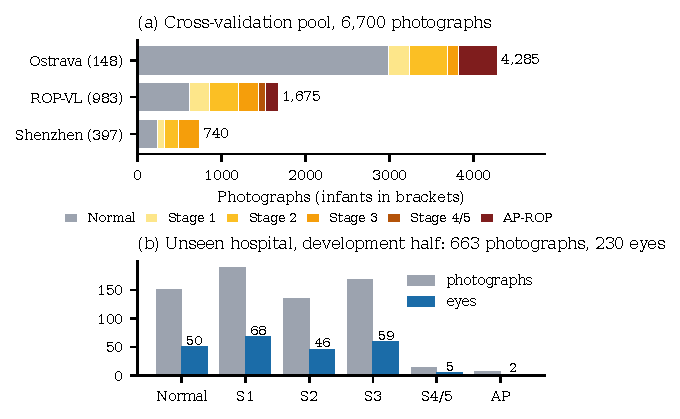
\includegraphics[width=\columnwidth]{fig_dataset.pdf}
\caption{Data. (a) Cross-validation pool by hospital and stage. (b) The unseen hospital's development half: photographs and eyes by stage.}
\label{fig:data}
\end{figure}

\subsection{Reference standard}
Labels are those released by the source institutions, graded by their clinicians against ICROP; we did not re-grade, and we treat this as the study's principal limitation. The unit a label describes differs by cohort and is respected in evaluation: Ostrava is scored per examination session, ROP-VL per eye examination, Shenzhen per photograph, and the unseen hospital per eye.

\subsection{Splits and pre-registration}
Folds are patient-grouped (five-fold, stratified by class) and shared by every arm. A protocol fixing the arms, parity rules, units, selection rule, primary endpoint, secondary endpoints, bootstrap, duplicate exclusion and minimum detectable difference was committed to version control on 19 October 2026, before any new model was trained. Five dated amendments, each committed before the experiment it governs, added the probe-chosen learning rates and the later arms; amendments 3--5 were written after earlier arms' cross-validation and development results were known, which they state. No selection used the unseen hospital.

\subsection{Arms A--G}
All arms share preprocessing (circle-crop, letterbox, CLAHE, 392~px), class-balanced cross-entropy ($\beta=0.999$)~\cite{cui2019} with label smoothing 0.05, strong and site-randomising augmentation, batch 16, 20 epochs, AdamW (weight decay 0.05), a one-cycle cosine schedule, mixed precision, last-epoch weights, no early stopping, and seeds 42 and 1337. Only the backbone, input size, normalisation and learning-rate recipe may differ.
\begin{itemize}
\item \textbf{A, retinal:} RETFound-Green ViT-S/14 with four register tokens (21.8~M parameters)~\cite{engelmann2025}, average pooling, a fresh six-way head, normalisation 0.5/0.5.
\item \textbf{B, natural:} DINOv2 ViT-S/14-reg~\cite{oquab2024}, the identical architecture, ImageNet normalisation.
\item \textbf{C, baseline:} EfficientNetV2-S~\cite{tan2021} from~\cite{nagpure2026}, scored from its saved predictions, never re-inferred.
\item \textbf{D, examination-level training:} B with a log-sum-exp loss over $K\le8$ frames of each Ostrava session, $\mathbf{z}=\tau\log\sum_k\exp(\mathbf{z}_k/\tau)$, $\tau=1$, scored against the session label; other cohorts keep per-photograph loss.
\item \textbf{E, ensemble:} the mean of A, B and C's probabilities, matched by seed.
\item \textbf{F, adaptation:} B with self-ensembling~\cite{french2018}: an EMA teacher (decay 0.99) scores unlabelled photographs of the unseen hospital's development half, and the student is penalised where the teacher is $\ge0.90$ confident; labels are never read; F's development numbers are therefore transductive.
\item \textbf{G, native resolution:} B at 518~px.
\end{itemize}
Transformers use layer-wise learning-rate decay 0.8, drop-path 0.1 and head dropout 0.3. The peak learning rate was chosen per arm by a probe on an inner patient-disjoint split of fold 0's training rows ($2\times10^{-4}$ for A, $10^{-4}$ for B; the rule kept $10^{-4}$ unless beaten by more than 0.03 macro-F1). All sessions ran on Kaggle T4 GPUs at about 33~min per fold for 392~px.

\subsection{Data audit, recipe and arms H and I (Amendment 5)}
After the A--G results and before any further run, Amendment 5 fixed one final round (v4; A--G form v3) on the selected arm B; A--G were frozen. The audit changes training rows only: the folds, the validation rows and the 14 exclusions are unchanged, so every arm is scored on the same 6{,}686 photographs. (1)~\emph{Ostrava frame quality}, judged within each camera: a frame fails if it is empty, below its camera's 10th percentile of Laplacian variance, or outside its camera's 2.5th--97.5th percentiles of luminance. A first rule took its thresholds, including a field-of-view minimum, from the two single-photograph hospitals; the audit showed that it measured the camera, not the frame (its field-of-view minimum failed 903 of 911 frames of one camera, among them all 125 Ostrava stage-3 frames), and a dated revision replaced it before the pool was built. (2)~\emph{Cap re-ranking}: the per-infant caps keep the sharpest passing frames, with a floor of two frames per infant and class. (3)~\emph{Near-duplicates}: both members of a cross-fold pair at 256-bit dHash distance $\le4$ and mean absolute pixel difference $\le5$ grey levels leave training. The quality rule removed 584 of 4{,}285 Ostrava frames (13.6\%) from the candidates; 439 of the 715 Ostrava training rows left and 418 sharper frames entered, and the v4 training pool holds 3{,}083 photographs (v3: 3{,}112; stage 1: 515 to 497). The duplicate rule removed 8 photographs, all among the 14 exact duplicates already excluded, and sent 14 different-label pairs to a clinician list without relabelling.

\textbf{H} is B's recipe on the v4 pool. \textbf{I} adds a recipe fixed in the amendment, nothing tuned: an exponential moving average (EMA) of the weights (decay 0.999, evaluated and saved), one epoch of head-only warm-up, rotation $\pm180^\circ$, crop scale 0.85--1, gamma $U(0.7,1.4)$ ($p=0.5$), Gaussian noise $\sigma=0.02$ ($p=0.3$), a Fourier amplitude swap of the central $3\times3$ low-frequency block with a random batch partner ($p=0.5$), and label smoothing 0.10. Leave-one-source-out (LOSO) folds train on two pool cohorts and score every photograph of the third: Shenzhen (the existing site fold), Ostrava and ROP-VL. Stage 4/5 exists only in ROP-VL, so its fold scores that stage untrained. B was run on the two new LOSO folds; H and I on all eight folds, with both seeds. A pre-run note, committed before any v4 kernel, disclosed two implementation details: a class absent from a fold's training rows now receives zero class-balanced weight (its count had been clamped to one, which made it the heaviest class; only the ROP-VL LOSO fold is affected, and no A--G weight changes), and I's EMA, started without warm-up, keeps about 5\% of the initial weights on a cross-validation fold (17\% on the ROP-VL LOSO fold).

\begin{table*}[!t]
\caption{Headline results, pooled over two seeds. QWK on the 5-class map with 95\% infant-clustered CI; LOSO = mean QWK over the three leave-one-cohort-out folds (Amendment 5c guard); accuracy and macro-F1 over present classes.}
\label{tab:main}
\centering\small
\begin{tabular}{@{}lcccc@{}}
\toprule
Arm & CV QWK (CI) & LOSO & Eye QWK, unseen hospital (CI) & Eye acc.\ / macro-F1\\
\midrule
A retinal ViT-S & 0.794 (0.664--0.915) & -- & 0.774 (0.707--0.828) & 0.632 / 0.563\\
B natural ViT-S & \textbf{0.825} (0.737--0.911) & 0.834 & 0.756 (0.679--0.821) & 0.630 / 0.566\\
C EfficientNetV2-S & 0.816 (0.713--0.916) & -- & 0.760 (0.680--0.822) & 0.624 / \textbf{0.573}\\
D B + exam loss & 0.797 (0.699--0.909) & -- & 0.746 (0.671--0.810) & 0.609 / 0.542\\
E ensemble A+B+C & 0.821 (0.708--0.927) & -- & 0.770 (0.697--0.827) & \textbf{0.639} / 0.568\\
F B + adaptation$^\dagger$ & 0.812 (0.704--0.915) & -- & 0.744 (0.665--0.812) & 0.624 / 0.551\\
G B at 518 px & 0.814 (0.706--0.915) & -- & 0.767 (0.697--0.827) & 0.627 / 0.551\\
H B on the v4 pool & 0.813 (0.707--0.914) & \textbf{0.842} & 0.750 (0.674--0.814) & 0.620 / 0.556\\
I B, v4 pool + recipe & 0.821 (0.727--0.912) & 0.839 & \textbf{0.776} (0.705--0.834) & 0.633 / 0.560\\
\bottomrule
\end{tabular}
\par\smallskip\footnotesize $^\dagger$transductive: F saw the unseen hospital's photographs without labels. LOSO was run for B, H and I only.
\end{table*}

\begin{figure*}[!t]
\centering
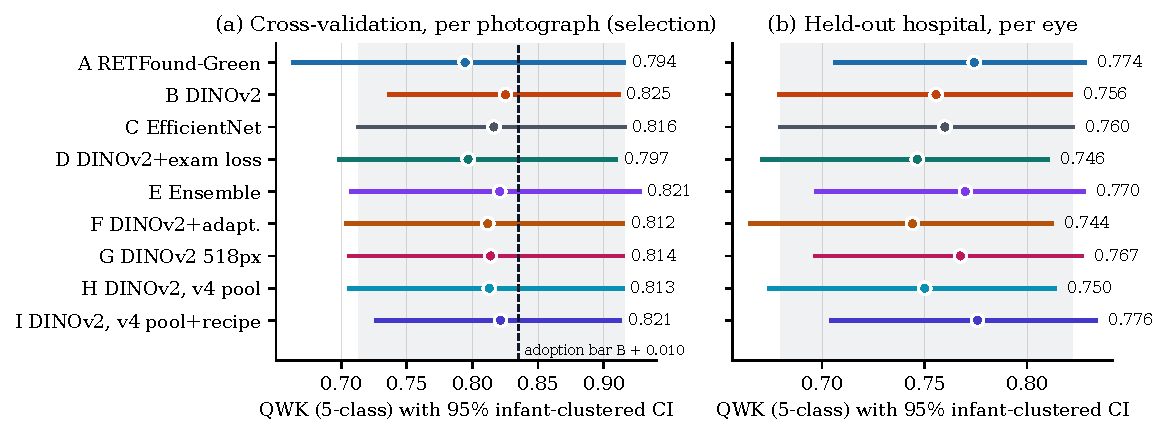
\includegraphics[width=\textwidth]{fig_compare.pdf}
\caption{QWK of the nine arms with 95\% infant-clustered intervals. (a) Cross-validation per photograph, the selection metric; dashed: the Amendment 5c adoption bar for H and I (B $+$ 0.010). (b) The unseen hospital per eye. The shaded band is the baseline's interval; every arm lies inside it.}
\label{fig:compare}
\end{figure*}

\subsection{Eye-level inference}
Each photograph receives a probability vector; the eye's stage is the most severe predicted stage over its photographs (the clinical reading rule), the photograph attaining it is the driving photograph, and its vector is the eye's vector. The any-ROP score of an eye is $\max_i(1-p_{i,\text{normal}})$. A learned attention aggregator was tried on frozen features before the design and lost to this rule on the unseen hospital ($-0.080$ QWK, CI excluding zero), so it was not pursued.

\subsection{Endpoints and statistics}
Selection rule (A--G): cross-validation pooled out-of-fold image QWK on the five-class map (AP-ROP folded onto stage 4/5), computed once per arm. Amendment 5c: adopt I if its cross-validation QWK exceeds B's by at least $+0.010$ and its mean LOSO QWK over the three held-out cohorts is no more than 0.010 below B's; else H under the same two conditions; else B stays. Primary endpoint (locked half, pending, now for A--I together): eye-level QWK, A$-$C. Secondary (Holm): A$-$B, D$-$A, E$-$C, F$-$B, G$-$B; Amendment 5 added H$-$B, I$-$B and I$-$H. Descriptive: accuracy, macro-F1 over present classes, per-class recall, confusion matrices, any-ROP sensitivity and specificity at the operating point fixed on cross-validation at 90\% unit sensitivity, calibration (ECE, Brier, NLL) after one temperature fitted on cross-validation eye-level vectors, and per-cohort unit-level QWK. Intervals are 95\% percentile bootstrap over 2{,}000 resamples of infants with each arm's prediction lists (two seeds; ten fold checkpoints on the unseen hospital) averaged inside each replicate; paired differences use the same resample. The minimum detectable eye-level difference at 80\% power on 230 eyes is about 0.08.

\section{Results}
\begin{figure*}[!t]
\centering
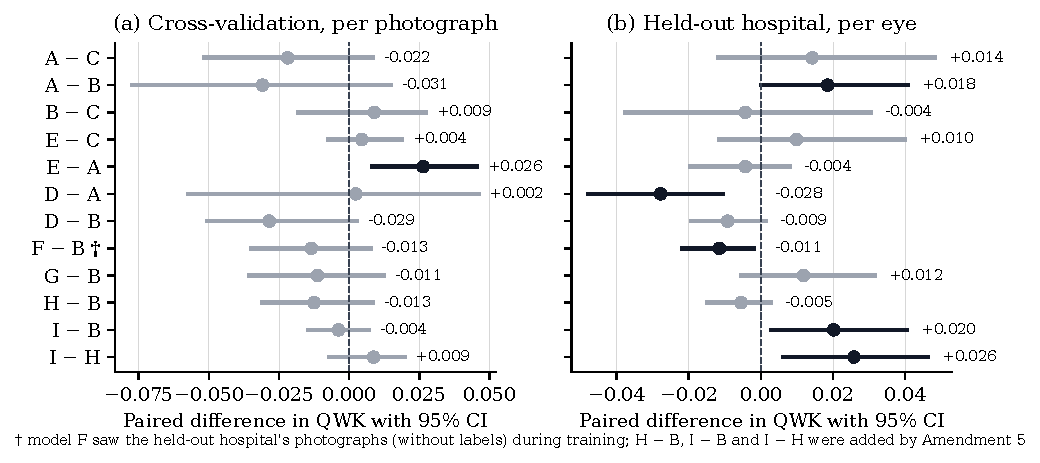
\includegraphics[width=\textwidth]{fig_contrasts.pdf}
\caption{Paired contrasts, both arms scored on the same infant resample; black: interval excludes zero (cross-validation: E$-$A; unseen hospital: D$-$A and F$-$B below zero, A$-$B, I$-$B and I$-$H above). H$-$B, I$-$B and I$-$H were added by Amendment 5.}
\label{fig:contrasts}
\end{figure*}

\subsection{Selection and the pre-training contrast}
Table~\ref{tab:main} and Fig.~\ref{fig:compare} give the headline results. The selection rule chose B (cross-validation QWK 0.825, 95\% CI 0.737--0.911) over A (0.794) and C (0.816). On the unseen hospital, per eye, A scored 0.774 (0.707--0.828), B 0.756 (0.679--0.821) and C 0.760 (0.680--0.822). Fig.~\ref{fig:contrasts} shows every paired contrast: A$-$C $+0.014$ ($-0.012$ to $+0.048$), A$-$B $+0.018$ ($0.000$ to $+0.041$), B$-$C $-0.004$ ($-0.038$ to $+0.030$), all below the stated minimum detectable difference. In cross-validation A$-$B was $-0.031$ ($-0.077$ to $+0.015$): the sign of the retinal-versus-natural difference reverses between the training hospitals and the unseen one. Across all nine arms, cross-validation QWK spans 0.794--0.825 and eye-level QWK at the unseen hospital 0.744--0.776, against single-arm intervals 0.12--0.25 wide.

\subsection{Data audit and recipe (arms H and I)}
\begin{figure*}[!t]
\centering
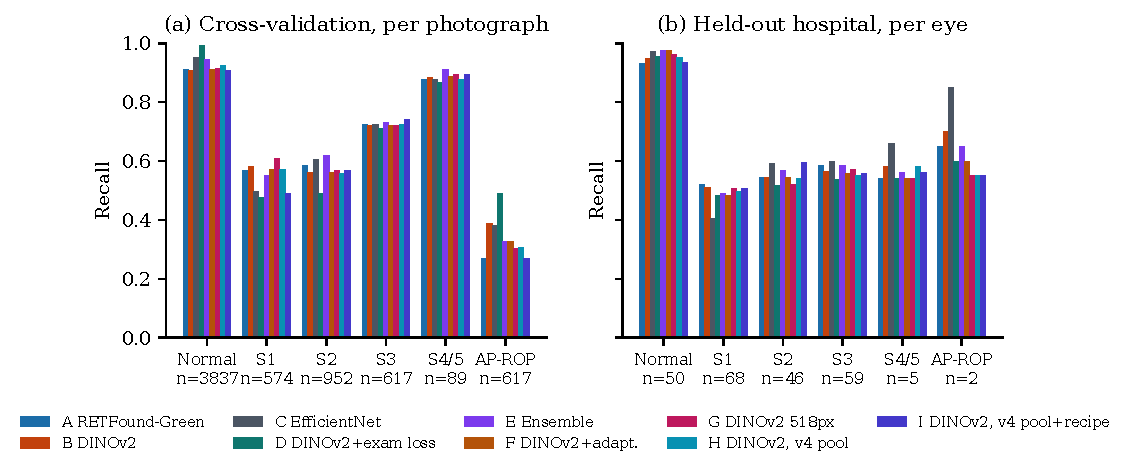
\includegraphics[width=\textwidth]{fig_stage_recall.pdf}
\caption{Recall by stage for every arm. The transformers gain on stage 1 at the unseen hospital; the baseline keeps AP-ROP; I's cross-validation AP-ROP and stage-1 recall are the lowest.}
\label{fig:stage}
\end{figure*}

\begin{figure*}[!t]
\centering
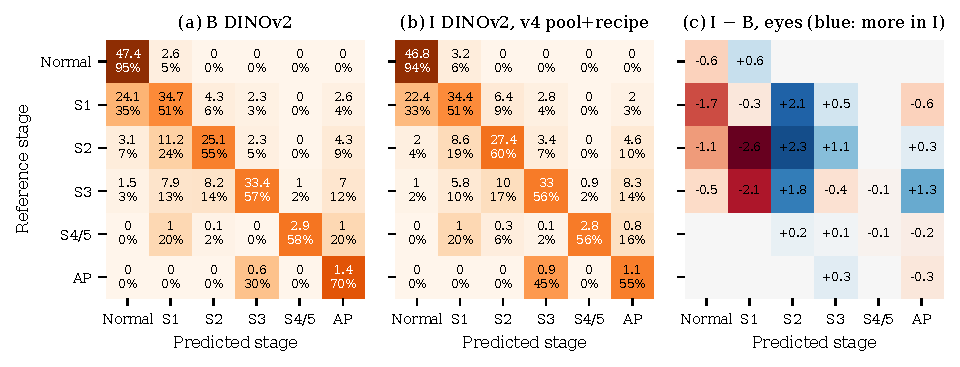
\includegraphics[width=\textwidth]{fig_confusion_BI.pdf}
\caption{Eye-level confusion matrices at the unseen hospital (230 eyes; counts averaged over each arm's ten checkpoints, row shares). (a) The selected arm B. (b) Arm I. (c) I minus B: I shifts predictions away from normal and stage 1 towards stages 2 and 3.}
\label{fig:cm}
\end{figure*}

Neither v4 arm met the adoption rule (Table~\ref{tab:main}, Fig.~\ref{fig:compare}a): in cross-validation, I$-$B was $-0.004$ ($-0.015$ to $+0.007$) and H$-$B $-0.013$ ($-0.031$ to $+0.009$), both intervals wholly below the $+0.010$ bar. Both passed the LOSO guard (mean LOSO QWK: B 0.834, H 0.842, I 0.839; Fig.~\ref{fig:loso}), so B stays the selected arm. The LOSO folds differ most where the cohort is hardest to transfer to: with Ostrava held out, QWK was 0.740 (0.398--0.845) for B, 0.766 for H and 0.779 for I, intervals 0.40--0.45 wide because 148 infants supply 4{,}285 photographs; with Shenzhen held out I fell to 0.942 (0.926--0.956) against B's 0.962 (0.953--0.971).

At the unseen hospital, which does not enter the rule, I scored 0.776 (0.705--0.834): I$-$B $+0.020$ ($+0.003$ to $+0.041$) and I$-$H $+0.026$ ($+0.006$ to $+0.046$), whereas H$-$B was $-0.005$ ($-0.015$ to $+0.003$). With A$-$B (lower bound 0.000), these are the only unseen-hospital contrasts whose intervals lie above zero (Fig.~\ref{fig:contrasts}). The gain is in QWK only: eye-level macro-F1 I$-$B was $-0.005$ ($-0.057$ to $+0.033$), and in cross-validation I lost macro-F1 ($-0.035$, $-0.053$ to $-0.001$). I was also better calibrated as trained (eye-level ECE 0.061 against 0.157 for B), consistent with EMA and stronger label smoothing.

The cross-validation cost falls on AP-ROP, whose recall fell from 0.389 (B) to 0.306 (H) and 0.269 (I). The fall sits in fold 0, where 470 of the 476 AP-ROP validation photographs are frames of one Ostrava infant's examinations, scored by models that never train on an Ostrava AP-ROP frame. Fold-0 AP-ROP recall was 0.246, 0.142 and 0.101 for B, H and I, and the two seeds of B differ there by 0.160; on folds 1--4, whose AP-ROP photographs come from ROP-VL infants, the arms reach 0.866, 0.859 and 0.835. Both pools hold the same 168 AP-ROP training photographs. The drop therefore measures how the rest of the pool shifts the reading of one infant's near-identical frames, which share one examination label: a label-unit artefact, not lost AP-ROP data.

\begin{figure}[!t]
\centering
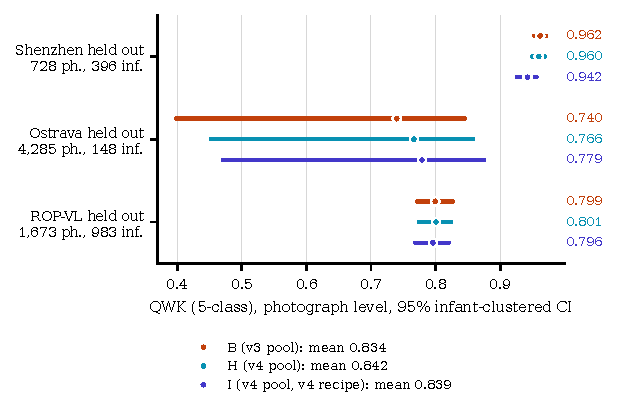
\includegraphics[width=\columnwidth]{fig_loso.pdf}
\caption{Leave-one-source-out folds: each model trains on two cohorts and is scored on every photograph of the third (both seeds pooled). B trains on the v3 pool, H and I on the v4 pool; the ROP-VL fold scores stage 4/5 with no training example.}
\label{fig:loso}
\end{figure}

\subsection{Per-stage behaviour}
Fig.~\ref{fig:stage} and Fig.~\ref{fig:cm} show where the arms differ. Stage-1 eye recall at the unseen hospital is 0.52 (A), 0.51 (B, G, I) and 0.50 (H) against 0.40 (C); in cross-validation it is 0.57--0.61 for A, B, F, G and H against 0.50 for C, and 0.49 for I, whose recipe, not its pool, costs stage-1 recall (H shares I's pool and keeps 0.57). I's eye-level gain comes from stage 2 (recall 0.60 against 0.55 for B) and from fewer stage-1 eyes called normal. Errors are between adjacent stages: for B, 24 of 68 stage-1 eyes are called normal and 11 of 46 stage-2 eyes are called stage 1; two-stage errors are rare. Stage 4/5 and AP-ROP have 5 and 2 eyes at the unseen hospital and are not interpretable there.

\subsection{Training at the label's unit}
Scored at each training cohort's own unit, on Ostrava examinations D scored QWK 0.846 (95\% CI 0.692--0.917) against 0.701 (0.490--0.776) for B, the same encoder trained per photograph, 0.775 for C, and 0.710 and 0.712 for H and I. A post-hoc paired bootstrap over the 342 sessions (148 infants; 64 diseased sessions from 18 infants) gives D$-$B $+0.145$ ($+0.094$ to $+0.257$) in QWK and $+0.214$ ($+0.099$ to $+0.327$) in macro-F1; D$-$C $+0.071$ ($+0.015$ to $+0.230$). On ROP-VL eye examinations and Shenzhen photographs, whose labels are already per photograph, D is within noise of B, and at the unseen hospital D is slightly below A ($-0.028$, $-0.048$ to $-0.011$). D also gives Ostrava a larger share of optimiser steps (36\% against 22\%), a confound of the alternating batch design that we cannot separate here.

\subsection{Negative results}
\textbf{Resolution.} G at DINOv2's native 518~px ties B ($+0.012$, $-0.005$ to $+0.032$ per eye) and raises stage-1 recall only in cross-validation (0.61 against 0.58), not at the unseen hospital (0.51 against 0.51). \textbf{Ensemble.} E ties C ($+0.010$, $-0.012$ to $+0.040$). \textbf{Ordinal decoding.} A four-threshold decoder on the expected stage, cross-fitted on out-of-fold predictions, lowered cross-validation QWK for A and B by about 0.04 and Ostrava session QWK for every arm by 0.08--0.15; a post-hoc check attributes the first to fold 0, which holds 77\% of AP-ROP photographs so that cut points fitted with it do not transfer, and the second to the decoder collapsing the stage-1 band so that the worst-view rule over many frames calls normal sessions stage 2. Argmax remained the primary decode as pre-registered. \textbf{Adaptation.} F was slightly worse than B at the unseen hospital ($-0.011$, $-0.022$ to $-0.002$) although it had seen those photographs: with label smoothing and class weights the teacher's attainable confidence for normal, stage 1 and stage 2 is below 0.90, so the mask admitted about 8\% of photographs by the final epoch, nearly all severe-stage, and never reached the stage-1 boundary. \textbf{Transfer of the operating point and temperature.} The any-ROP threshold set at 90\% sensitivity on cross-validation reached 64--68\% sensitivity at the unseen hospital for every arm (specificity 1.00). Every cross-validation temperature sharpened (0.62--0.94), and it raised eye-level ECE at the unseen hospital for every arm, to 0.20--0.24; I's as-trained 0.061 became 0.196 (Fig.~\ref{fig:cal}).

\begin{figure}[!t]
\centering
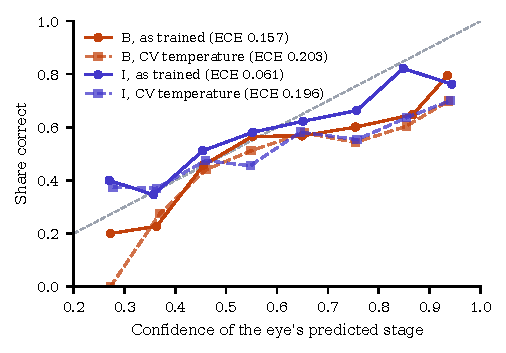
\includegraphics[width=\columnwidth]{fig_calibration.pdf}
\caption{Reliability per eye at the unseen hospital for B and I, as trained and after each arm's cross-validation temperature. B is over-confident as trained and I close to the diagonal; the temperature makes both more over-confident.}
\label{fig:cal}
\end{figure}

\section{Discussion}
Under a matched recipe, retinal pre-training did not beat natural-image pre-training for ICROP-3 staging, and with the backbone fixed, neither did a cleaner pool nor a stronger recipe: nine arms lie within 0.032 QWK of one another in cross-validation and at an unseen hospital. The selection metric did not move, and the one descriptive gain is below what this design can confirm.

The pre-training null extends ROP-Bench's binary, unmatched finding~\cite{luo2026} to multi-class staging with the architecture confound removed, and agrees with Mahboob et al.'s staging result with RETFound~\cite{mahboob2025}: once fine-tuning is allowed, the pre-training domain makes little difference at this scale of data. The sign of A$-$B reverses between cross-validation and the unseen hospital and neither reaches the minimum detectable difference.

The data audit changed what the models trained on: the quality rule removed 584 Ostrava frames, and 439 of 715 Ostrava training rows were replaced by sharper frames. Cross-validation moved by $-0.013$ (H) and $-0.004$ (I), and the LOSO guard by $+0.009$ and $+0.005$. Sharper frames carry the same examination labels as the frames they replace, so cleaning the images cannot remove the label noise of frames that do not show the finding; D's examination-level loss, which addresses exactly that, moved Ostrava examinations by 0.145. I's gain at the unseen hospital ($+0.020$) fits what its regularisers target, camera and illumination shift, and I was the best calibrated arm as trained. But the gain is descriptive: the development half has now been examined for nine arms, the interval's lower bound is $+0.003$, and the protocol's minimum detectable difference for the locked half is 0.08, so even the locked scoring cannot confirm an effect of this size. Its costs, lower cross-validation macro-F1, stage-1 and AP-ROP recall, are real, and the AP-ROP part is itself a label-unit artefact: one Ostrava infant's 470 frames carry one examination label and decide fold 0.

What remains is a ceiling set by the labels. The errors are adjacent-stage confusions, normal/stage 1 and stage 1/stage 2, which is where human experts disagree most~\cite{gschliesser2015,campbell2016}. A model trained on three institutions' reading of the stage-1 boundary cannot agree with a fourth institution's reading better than experts agree with each other; our unweighted eye-level kappa (0.52 for B, 0.53 for I) already exceeds the published inter-expert value (0.24), with the caveat that these are different quantities on different images. Lan et al.'s feature-level fusion over five fixed fields of view~\cite{lan2026} suggests that a learned eye-level aggregator can beat an outcome-level rule when eye-level labels exist for training; our attempt lost to the worst-view rule because our only multi-photograph training bags are mostly normal Ostrava sessions. Eye-level training labels, not another recipe, are the missing input.

The large effect was not architectural. Training at the examination session, the unit Ostrava's labels describe, raised examination-level agreement by 0.145 and did nothing elsewhere, because elsewhere the labels are already per photograph. When a label is a property of a session, per-photograph training teaches the model to call non-showing frames diseased, and per-session pooling lets the most abnormal frame carry the label. The i-ROP group's examination-level evaluation~\cite{brown2018,derks2025} and Peng et al.'s results~\cite{peng2021} point the same way; we add that the unit belongs in the loss, not only in the metric, and give its size. The result is post hoc, rests on 18 diseased infants and is confounded with Ostrava's share of training steps, so it is a hypothesis for a pre-registered follow-up.

Clinically, the findings argue for three practices. The eye, not the photograph, is the unit to report, with the driving photograph shown. The screening threshold and the calibration must be set at the site of use, since neither transferred for any arm, including the best-calibrated one. And clinician re-grading of stage-1 photographs on which several independent models disagree with the label, with the 14 different-label near-duplicate pairs, is the step most likely to raise the ceiling.

This study has several limitations. First, labels were not re-graded and two cohorts label per examination, so some training labels describe frames that do not show the finding. Second, the severe classes have five and two eyes at the unseen hospital and cannot be evaluated there; AP-ROP in cross-validation is dominated by one infant. Third, the unseen hospital's development half was used for design decisions in our earlier work and has now been examined for nine arms, so its numbers are descriptive and any difference there is one look of many; the locked half, which carries the pre-registered primary endpoint, remains unscored and will be opened once, for A--I together, after approval. Fourth, F's numbers on that hospital are transductive. Fifth, amendments 3--5 were written after earlier arms' results were known; they add arms and endpoints but change no pre-registered one. Sixth, two seeds per arm bound seed variability only coarsely; fold-0 QWK differs by up to 0.08 between seeds. Seventh, B's LOSO folds ran after the v3 round on the v3 pool, and I's EMA retains 5--17\% of its initial weights.

\section{Conclusion}
Within a pre-registered, architecture-matched design, retinal and natural-image pre-training gave indistinguishable ICROP-3 staging at an unseen hospital, and neither beat an ImageNet convolutional baseline; the transformers improved stage-1 recall. A per-camera data audit and a regularising recipe did not move the selection metric; the recipe's gain at the unseen hospital was descriptive and below the detectable difference. Resolution, ensembling, decision rules and unsupervised adaptation did not move the eye-level result, and operating points did not transfer. Training at the unit the labels describe did move the result, by 0.145 kappa on the cohort labelled per examination. Future work is clinician re-grading of the stage-1 boundary and the single scoring of the locked half for all nine arms. For ROP staging, the next gains may lie in the labels and their units rather than in the backbone, the data cleaning or the recipe.

\section*{Compliance with Ethical Standards}
This retrospective study used only publicly released, de-identified datasets under their licences (Ostrava/RIDIRP, ROP-VL, Shenzhen, Multi-View ROP, CC BY-NC); no new data were collected and no ethical approval was required. RETFound-Green's weights are used under their non-commercial licence. The system is research software and not a medical device. No funding was received; the authors declare no conflicts of interest.

\section*{Acknowledgments}
We thank the releasing institutions and Kaggle for the free GPU time on which every model was trained. \FILL{venue-specific AI disclosure, e.g.: Claude (Anthropic) was used to draft and edit code and text in all sections under the authors' direction; the authors verified every number against the committed result files and take full responsibility for the content.}

\begin{thebibliography}{99}
\bibitem{icrop3} M.~F.~Chiang, G.~E.~Quinn, A.~R.~Fielder, \emph{et al.}, ``International classification of retinopathy of prematurity, third edition,'' \emph{Ophthalmology}, vol.~128, no.~10, pp.~e51--e68, 2021.
\bibitem{vahid2026} M.~Vahidmoghadam, P.~Ghorbani, M.~J.~Ahmadi, \emph{et al.}, ``Automated diagnosis of plus form and early stages of ROP using deep learning models,'' \emph{Sci. Rep.}, vol.~16, art.~7234, 2026.
\bibitem{wang2026} \FILL{author list}, ``VEA-Net: vascular enhancement attention network for multi-task retinopathy of prematurity classification,'' \emph{Front. Cell Dev. Biol.}, 2026.
\bibitem{luo2026} Luo, Guo, Chen, Liang, and Lin, ``ROP-Bench: a benchmark of foundation models for retinopathy of prematurity,'' Zenodo record 20721027, 2026. \FILL{confirm author list and title}
\bibitem{mahboob2025} Z.~Mahboob, A.~O.~Ahsan, and M.~Wilms, ``Using an adult retinal image analysis foundation model for retinopathy of prematurity staging: are there benefits?'' in \emph{Proc. SPIE Medical Imaging 2025: Computer-Aided Diagnosis}, 2025, p.~116, doi:10.1117/12.3047303. \FILL{confirm volume and paper number}
\bibitem{engelmann2025} J.~Engelmann, \emph{et al.}, ``RETFound-Green: a green retinal foundation model,'' \emph{Nat. Commun.}, 2025. \FILL{confirm title, volume, article number}
\bibitem{nagpure2026} P.~Nagpure, R.~Bait, P.~Rangnekar, Y.~Shengale, and A.~Kumar, ``What the label unit hides: an audited multi-hospital benchmark for ICROP retinopathy of prematurity staging,'' \FILL{preprint venue, DOI, 2026}.
\bibitem{peng2021} Y.~Peng, W.~Zhu, Z.~Chen, \emph{et al.}, ``Automatic staging for retinopathy of prematurity with deep feature fusion and ordinal classification strategy,'' \emph{IEEE Trans. Med. Imaging}, vol.~40, no.~7, pp.~1750--1762, 2021.
\bibitem{brown2018} J.~M.~Brown, J.~P.~Campbell, A.~Beers, \emph{et al.}, ``Automated diagnosis of plus disease in retinopathy of prematurity using deep convolutional neural networks,'' \emph{JAMA Ophthalmol.}, vol.~136, no.~7, pp.~803--810, 2018.
\bibitem{derks2025} \FILL{author list} and J.~P.~Campbell, ``External validation of the i-ROP deep learning system,'' \emph{J. AAPOS}, 2025. \FILL{confirm title, volume, pages}
\bibitem{wang2021} J.~Wang, J.~Ji, M.~Zhang, \emph{et al.}, ``Automated explainable multidimensional deep learning platform of retinal images for retinopathy of prematurity screening,'' \emph{JAMA Netw. Open}, vol.~4, no.~5, e218758, 2021.
\bibitem{lan2026} W.-H.~Lan, C.-L.~Tsai, and W.-C.~Wu, ``Optimizing field-of-view for type-1 retinopathy of prematurity via multiple instance learning,'' \emph{Transl. Vis. Sci. Technol.}, vol.~15, no.~8, art.~13, 2026, doi:10.1167/tvst.15.8.13.
\bibitem{chen2025} \FILL{author list}, ``SABPI-Net \FILL{full title},'' in \emph{Proc. MICCAI}, 2025.
\bibitem{zhao2026} Zhao and Li, ``DeepAdapter: self-supervised pre-training and domain adaptation for retinopathy of prematurity screening,'' \emph{Br. J. Ophthalmol.}, 2026, doi:10.1136/bjo-2025-328559. \FILL{confirm title and authors}
\bibitem{gschliesser2015} A.~Gschlie\ss{}er, E.~Stifter, T.~Neumayer, \emph{et al.}, ``Inter-expert and intra-expert agreement on the diagnosis and treatment of retinopathy of prematurity,'' \emph{Am. J. Ophthalmol.}, vol.~160, no.~3, pp.~553--560, 2015.
\bibitem{campbell2016} J.~P.~Campbell, S.~N.~Ryan, E.~Lore, \emph{et al.}, ``Diagnostic discrepancies in retinopathy of prematurity classification,'' \emph{Ophthalmology}, vol.~123, no.~8, pp.~1795--1801, 2016.
\bibitem{timkovic2024} J.~Timkovi\v{c}, \emph{et al.}, ``Retinal image dataset of infants and retinopathy of prematurity,'' \emph{Sci. Data}, vol.~11, art.~814, 2024.
\bibitem{oquab2024} M.~Oquab, T.~Darcet, T.~Moutakanni, \emph{et al.}, ``DINOv2: learning robust visual features without supervision,'' \emph{Trans. Mach. Learn. Res.}, 2024.
\bibitem{cui2019} Y.~Cui, M.~Jia, T.-Y.~Lin, Y.~Song, and S.~Belongie, ``Class-balanced loss based on effective number of samples,'' in \emph{Proc. IEEE/CVF CVPR}, 2019, pp.~9268--9277.
\bibitem{tan2021} M.~Tan and Q.~V.~Le, ``EfficientNetV2: smaller models and faster training,'' in \emph{Proc. ICML}, 2021, pp.~10096--10106.
\bibitem{french2018} G.~French, M.~Mackiewicz, and M.~Fisher, ``Self-ensembling for visual domain adaptation,'' in \emph{Proc. ICLR}, 2018.
\end{thebibliography}
\end{document}
